	\newpage
\section{Poradnik użytkowania}

Po zbudowaniu i uruchomieniu aplikacji zgodnie z instrukcją zawartą w pliku \texttt{README.md} w repozytorium projektu, użytkownik znajdzie się na stronie głównej aplikacji.

\subsection{Rejestracja}

\begin{figure}[H]
	\centering
	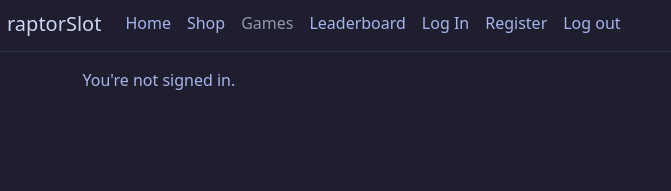
\includegraphics[width=1\textwidth]{images/tutorial/main_page.png}
	\caption{\centering{Strona główna aplikacji}}
\end{figure}

Dalej, użytkownik może skorzystać z pasku na górze strony, aby stworzyć nowe konto lub się zalogować.

\begin{figure}[H]
	\centering
	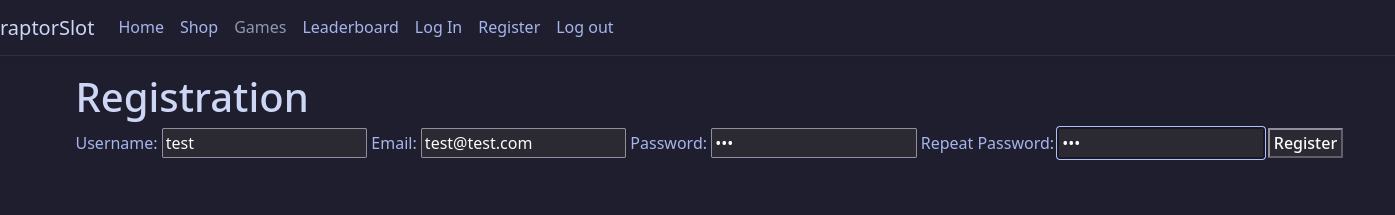
\includegraphics[width=1\textwidth]{images/tutorial/register.png}
	\caption{\centering{Strona rejestracji}}
\end{figure}

\subsection{Kupowanie żetonów i granie w gry}
Po zalogowaniu bądź rejestracji, użytkownik znowu zostanie przekierowany do strony głównej. Teraz jednak będzie posiadał dostęp do większości funkcjonalności aplikacji. Jeżeli użytkownik chce zagrać w jakąś grę, powinien najpierw kupić żetony w zakładce \texttt{Shop}

\begin{figure}[H]
	\centering
	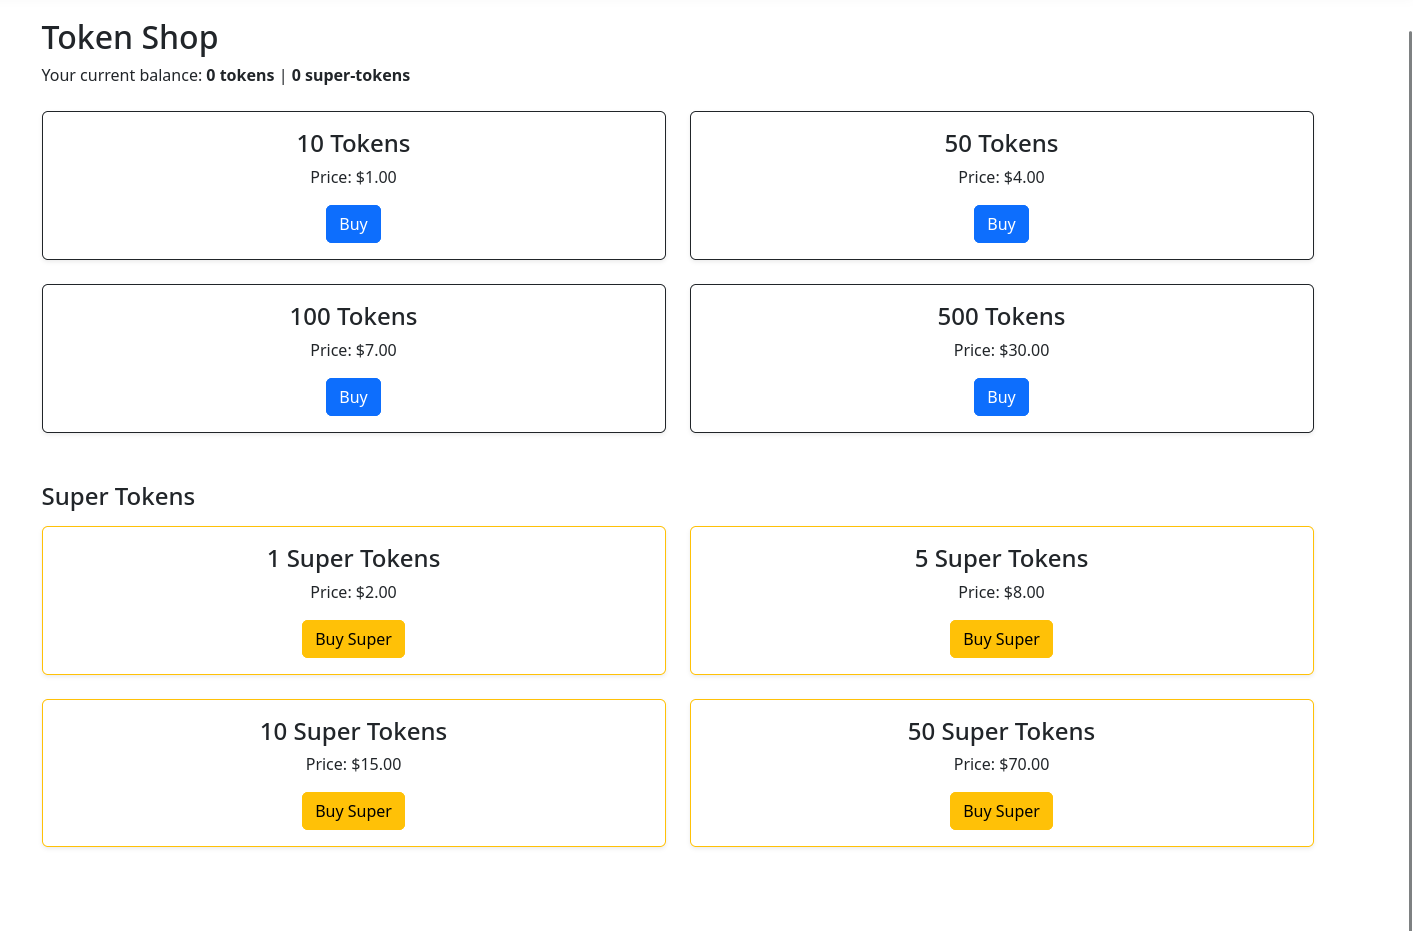
\includegraphics[width=1\textwidth]{images/tutorial/shop.png}
	\caption{\centering{Strona sklepu z żetonami}}
\end{figure}

Po zakupie żetonów, użytkownik może przejść do zakładki \texttt{Games}, gdzie znajdzie listę dostępnych gier. 

\todo{Dać screen z grami jak sie jezyk naprawi}

\todo{opis slotów i losowania liczby}

Ostatnią grą dostępną w aplikacji jest ruletka.

\begin{figure}[H]
	\centering
	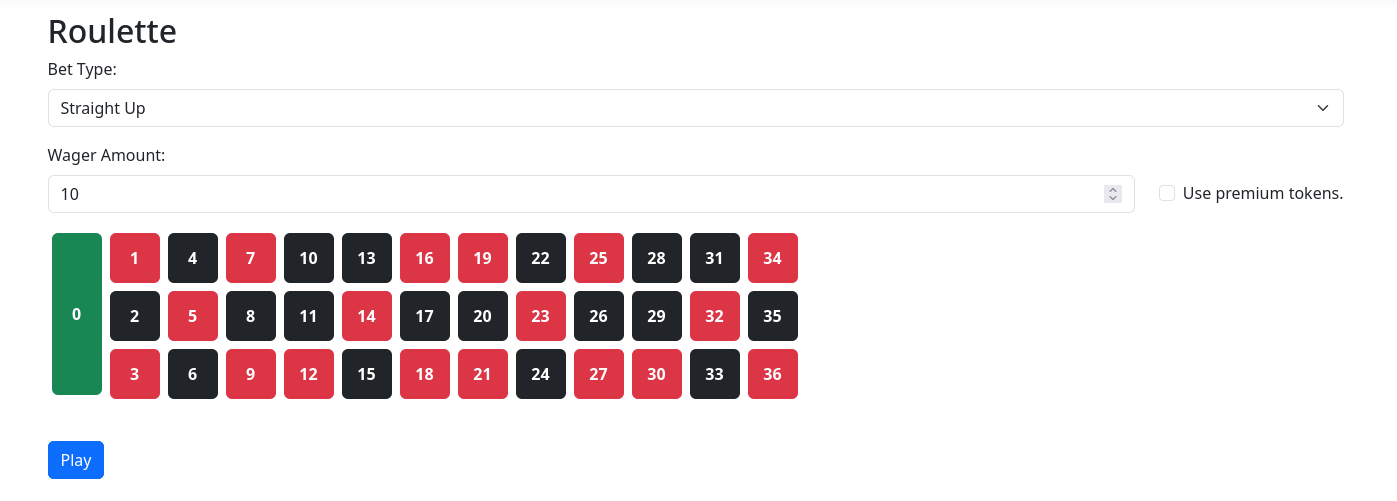
\includegraphics[width=1\textwidth]{images/tutorial/roulette.png}
	\caption{\centering{Strona gry w ruletkę}}
\end{figure}

Użytkownik może wybrać typ zakładu, kwotę do postawienia, liczby, bądź kolory na jakie chce postawić i czy chce używać żetonów premium. 

\begin{figure}[H]
	\centering
	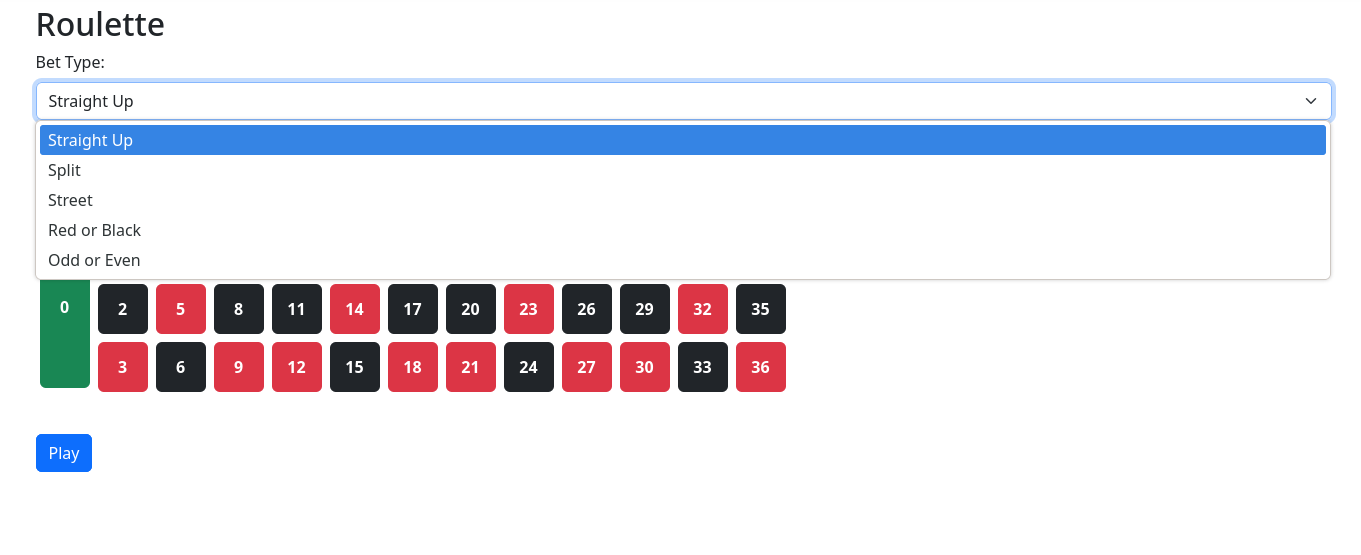
\includegraphics[width=1\textwidth]{images/tutorial/roulette_bet_types.png}
	\caption{\centering{Typy zakładów w ruletce}}
\end{figure}

Po postawieniu zakładu, użytkownik powinien kliknąć przycisk \texttt{Play}, aby wylosować wynik.

\begin{figure}[H]
	\centering
	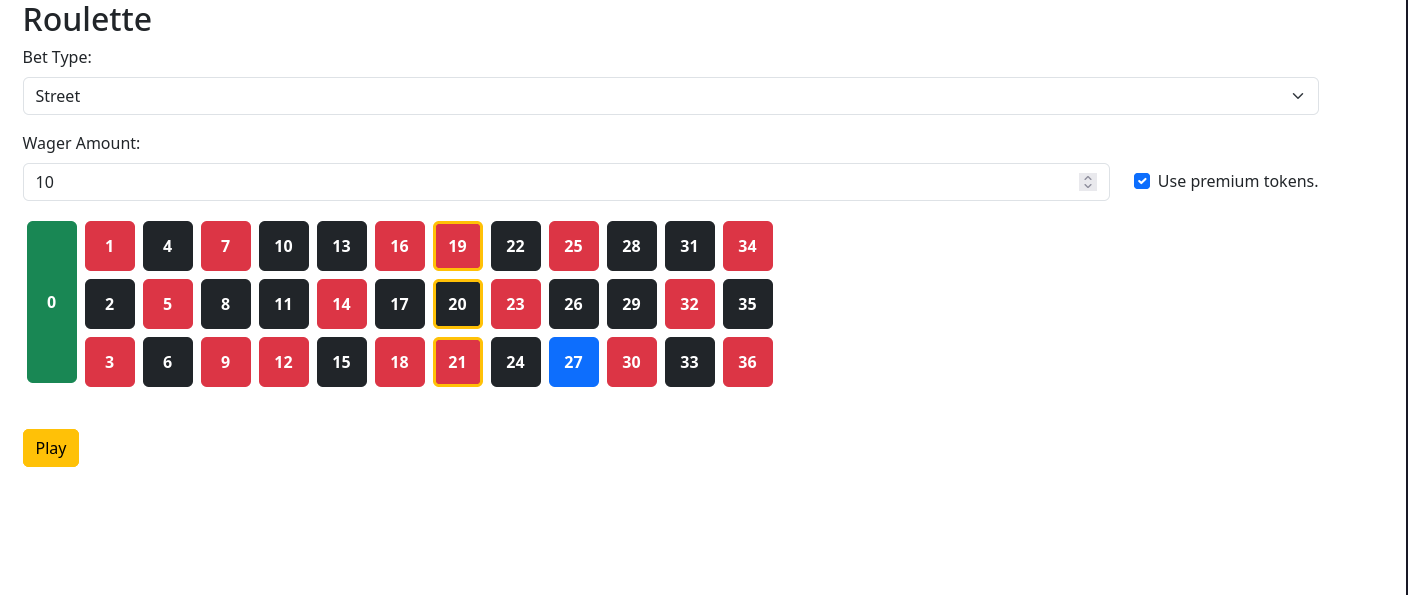
\includegraphics[width=1\textwidth]{images/tutorial/roulette_play.png}
	\caption{\centering{Losowanie wyniku w ruletce}}
\end{figure}

\begin{figure}[H]
	\centering
	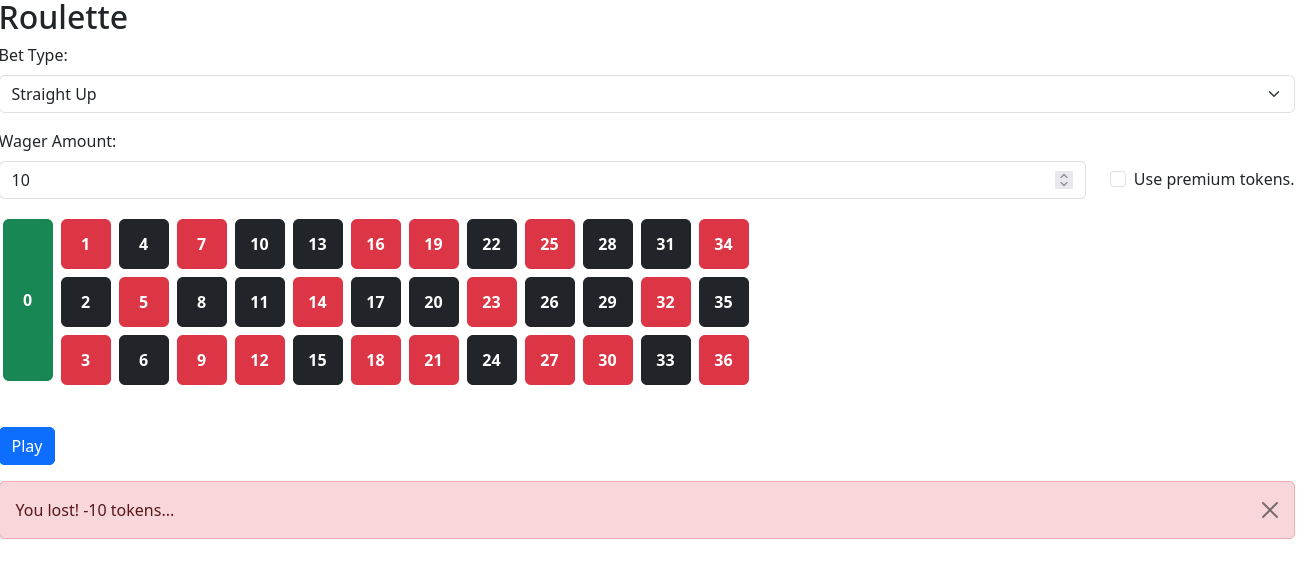
\includegraphics[width=1\textwidth]{images/tutorial/roulette_lost.png}
	\caption{\centering{Przegrana...}}
\end{figure}

\subsection{Zmiana awatara}

Na końcu topbrau storny znajduje się zakładka \texttt{Change User Avatar}, gdzie użytkownik może, jak nazwa wskazuje, zmienić swój awatar, klikając na przycisk \texttt{Browse}, a po wybraniu zdjęcia \texttt{Upload}.

\begin{figure}[H]
	\centering
	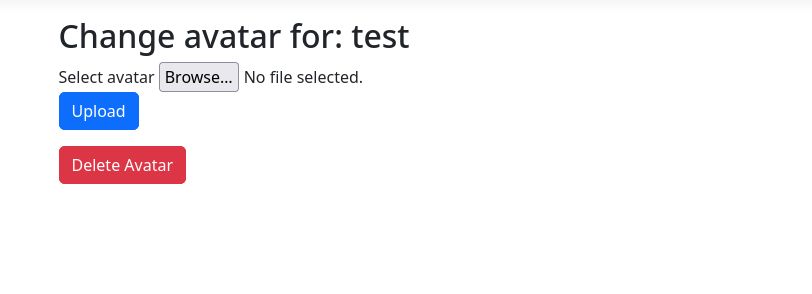
\includegraphics[width=1\textwidth]{images/tutorial/change_avatar.png}
	\caption{\centering{Strona zmiany awatara}}
\end{figure}

\begin{figure}[H]
	\centering
	
\includegraphics[width=1\textwidth]{images/tutorial/after_avatar.png}
	\caption{\centering{Topbar po zmianie awatara}}
\end{figure}

\subsection{Leaderboard}

Użytkownik może przeglądnąć też ranking graczy z największą ilością żetonów, klikając na zakładkę \texttt{Leaderboard} w topbarze.

\begin{figure}[H]
	\centering
	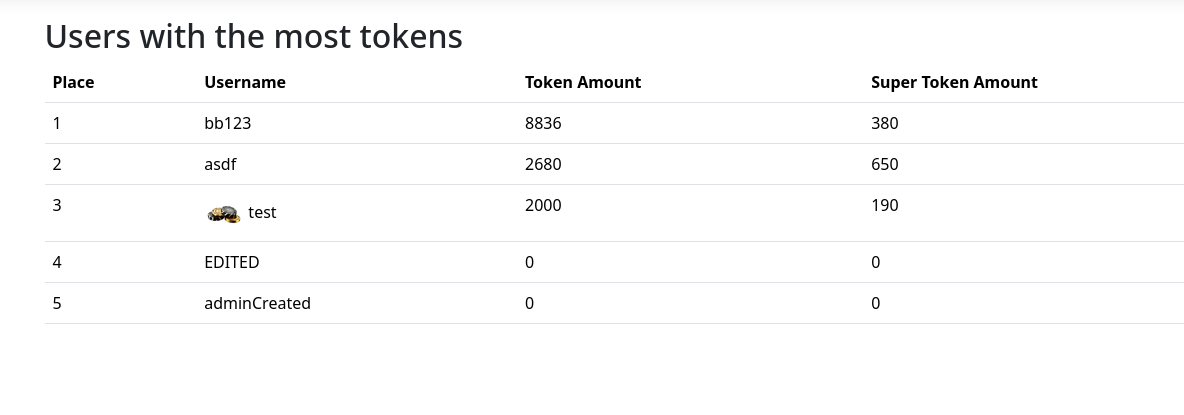
\includegraphics[width=1\textwidth]{images/tutorial/leaderboard.png}
	\caption{\centering{Strona rankingu graczy}}
\end{figure}

\subsection{Administracja}

\todo{}
